\documentclass{article}
\usepackage[margin=0.5in]{geometry}
\usepackage{listings}
\usepackage{color}
\usepackage{graphicx}
\usepackage{placeins}
\usepackage{fancyhdr}
\usepackage{wrapfig}
\begin{document}
\pagestyle{fancy}
\rhead{Ryan Morehart}

\title{Secure Software - Lab 8}
\author{Ryan Morehart}
\maketitle

\section{Task 1 - POP3 Password}
\par Cain actually failed to capture the password on my system (probably a misconfiguration on my part), but I went ahead and just pulled up wireshark. After starting the capture, I had Thunderbird pull mail from inbox.com using POP3 with no security. Filtering the resulting capture to just pop traffic, the password appears quite plainly:

\begin{figure}[h]
\centering
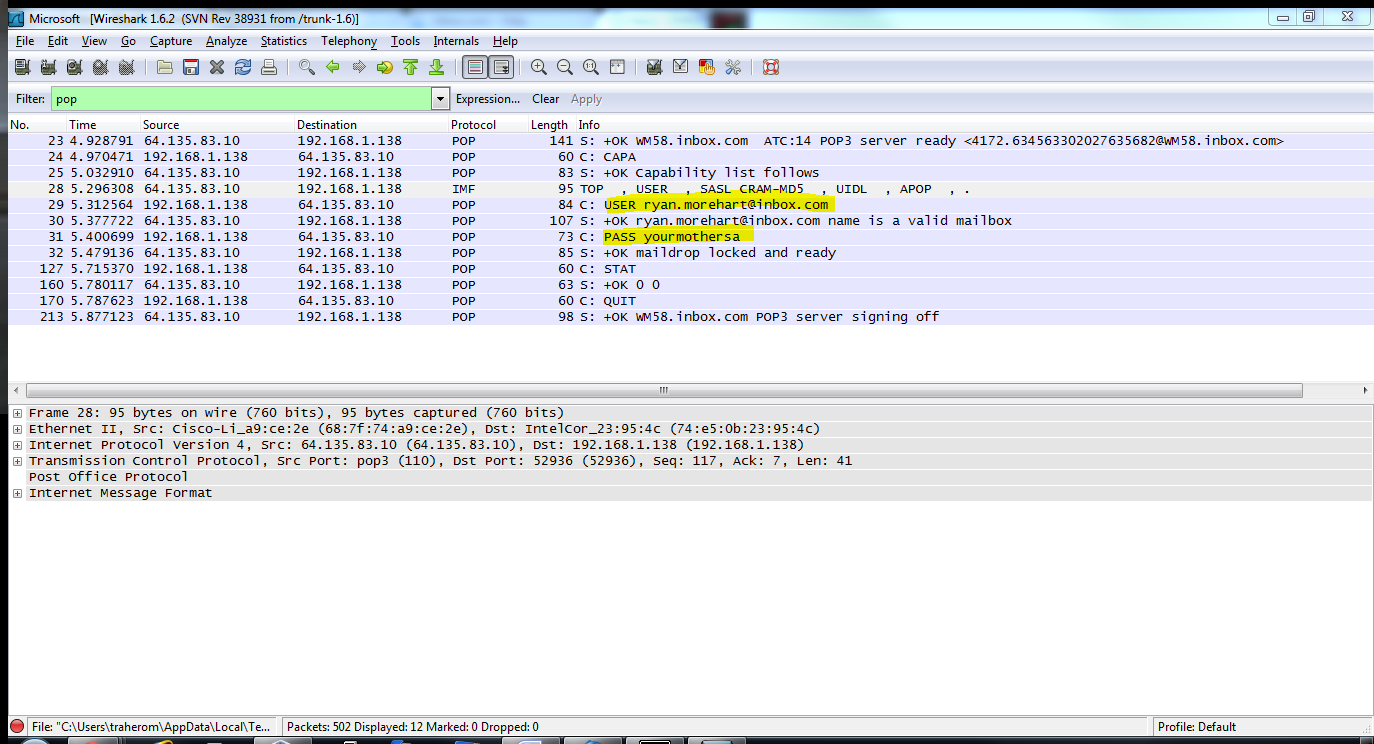
\includegraphics[width=0.9\textwidth, trim=0pt 300pt 200pt 50pt, clip]{pop3_password}
\caption{POP3 password}
\label{fig:pop}
\end{figure}

\par Obviously, the biggest problem with this is that the password is transmitted in the clear. Encrypted password authentation has been added to POP3, but this must be enabled to actually be effective.

\section{Task 2 - Bad Certificate}
\par When we first click the link from within Word, we first see this warning appear:
\begin{figure}[h]
\centering
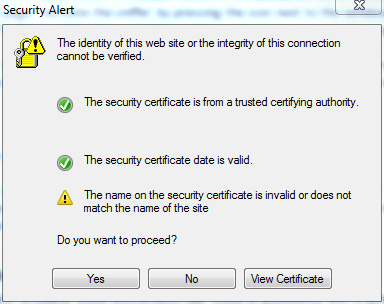
\includegraphics[]{first_warning}
\caption{Word 2007 Alert}
\label{fig:word_alert}
\end{figure}

\par Word has already nicely attempted to connect for us and found that the certificate was invalid. It is correctly signed, it just does not belong to jwart.co.uk.

\par If we still go to the site, Chrome then warns us of the danger, as seen in Figure \ref{fig:chromewarn}. This is a full-screen, blindingly obvious warning. However, Chrome does provide an easy way through (single click), so it may not deter many users.

\begin{figure}[h]
\centering
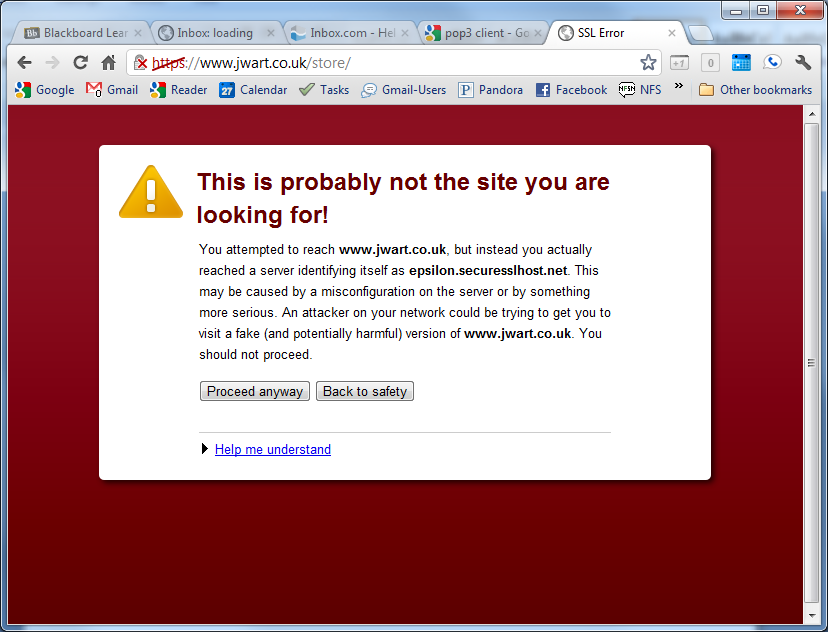
\includegraphics[width=0.9\textwidth, trim=0pt 125pt 0pt 30pt, clip]{chrome_warning}
\caption{Chrome Warning}
\label{fig:chromewarn}
\end{figure}

\par If we chose to proceed anyway, Chrome continues to warn us using the red/crossed out security icons (Figure \ref{fig:morewarnings}). The "insecure content" bar along the top of the page is actually mostly unrelated and is referring to content being loaded over HTTP instead of HTTPS like the main page.

\begin{figure}[h]
\centering
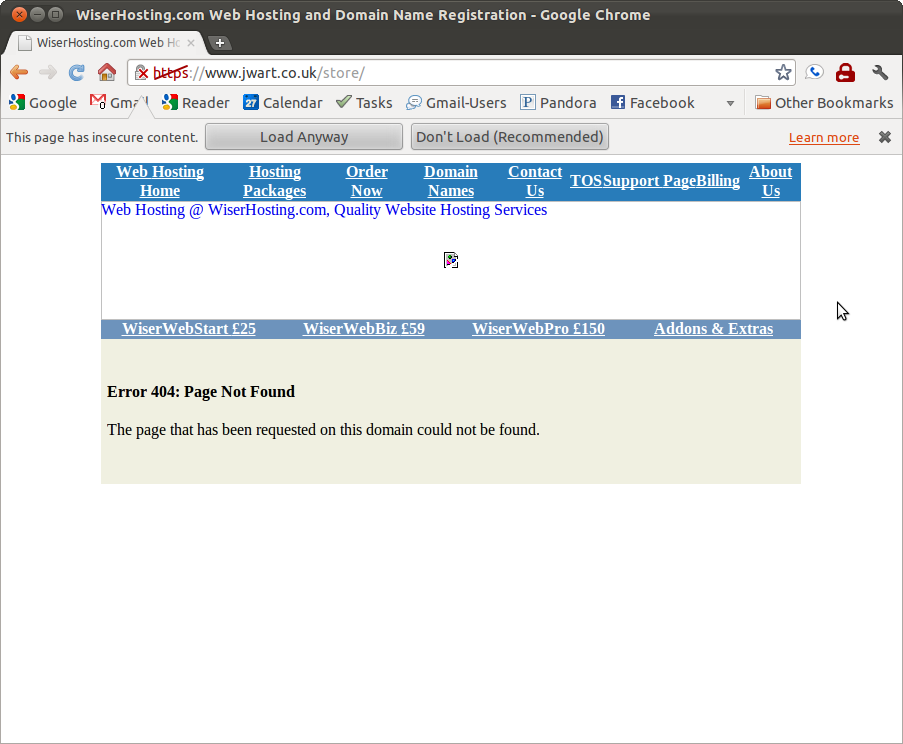
\includegraphics[width=0.9\textwidth, trim=0pt 300pt 200pt 50pt, clip]{insecure}
\caption{More security warnings from Chrome}
\label{fig:morewarnings}
\end{figure}

\par Looking at the certificate, it is validly signed and not expired. However, it belongs to a different domain (Figure \ref{fig:cert}).

\begin{figure}[h]
\centering
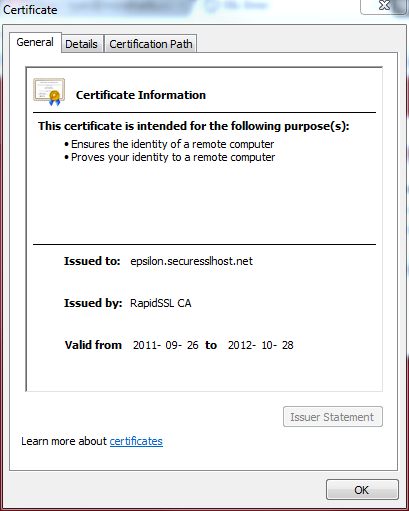
\includegraphics{cert}
\caption{Certificate Information}
\label{fig:cert}
\end{figure}

\par Ultimately I would not accept this certificate.

\end{document}

